\section{Analisi dei requisiti}
In questa sezione andremo a descrivere il modello funzionale del software
partendo da un analisi dei casi d'uso assegnati per l'applicativo, e proseguendo poi con tabelle cockburn e mock-up.
\subsection{Requisiti del software}
Lo sviluppo di Ratatouille23\texttrademark\ in parte è stato scandito dalla presenza di requisiti imposti dal cliente per il corretto funzionamento del software, in parte da requisiti tecnologici.

\subsubsection{Requisiti funzionali}
Il sistema offre le seguenti funzionalità:
\begin{enumerate}
  \item La possibilità da parte di un amministratore di poter creare utenze per i propri dipendenti (e.g. addetti alla sala, addetti alla cucina, supervisori) con nome utente scelto dall'aministratore ed una password di default.

  \item La possibilità da parte di un amministratore (o un supervisore) di personalizzare il menù dell'attività di ristorazione. In particolare, la possibilità di riordinare il menù, creare e/o eliminare elementi dal menù, caratterizzandoli tramite:
        \begin{itemize}
          \item \textit{nome}.
          \item \textit{descrizione}.
          \item \textit{elenco di allergeni comuni}.
          \item \textit{prezzo}.
        \end{itemize}
        In fase di creazione di un determinato piatto, è disponibile, utilizzando l'apposito tasto per la ricerca, l'autocompletamento di alcuni prodotti (e.g.: bibite o preconfezionati).
  \item La possibilità da parte di un addetto alla sala di poter registrare ordinazioni indicando l'identificativo del tavolo e gli elementi del menù (già presenti) desiderati.
  \item Un supervisore o un amministratore può inserire nel sistema degli avvisi (chiamati notifiche), che possono essere
        visualizzati da tutti i dipendenti. Ciascun dipendente può poi , qualora lo ritenesse necessario, marcare un avviso come “visualizzato” nascondendolo.
\end{enumerate}

\subsection{Requisiti non funzionali}
Le modalità secondo le quali saranno offerte le funzionalità sopracitate sono le seguenti:
\begin{itemize}
  \item \textbf{Usabilità} L'applicazione è stata sottoposta a una ricerca nel dettaglio di
        "User Personas".
  \item \textbf{Scalabilità}
        Scalabilità Il sistema deve avere un back-end in cloud scalabile per adattarsi a frequenze di accesso elevate.
  \item \textbf{Password policy security} Le password dell'utente verrano salvate in
        cloud con password crittografata.
  \item \textbf{Utilizzo di single-activity, multi-fragment} L'applicazione utilizza per
        fluidità e facile gestione il pattern di single-activity e multi-fragment in modo
        da dare precisi scopi alle activity che gestiscono fragment comuni.
\end{itemize}
\subsection{Requisiti di dominio}
\begin{itemize}
  \item \textbf{ISO/IEC} Il sistema deve essere conforme alle direttive \textit{ISO/IEC} del trattamento dei dati privati su servizi di hosting in cloud.
  \item \textbf{GDPR} Il sistema segue le direttive euorpee sulla \textit{GDPR} e quelle delle policy della privacy.
\end{itemize}
\subsection{Modellazione dei casi d'uso}
Di seguito sono descritti in dettaglio gli use-case scelti dal team di sviluppatori, al fine di dare un'idea concreta e chiara sul funzionamento del software sviluppato.
\subsubsection{Use-case generale}
Questo use-case è nato dopo aver attentamente valutato le richieste da parte degli stakeholders, infatti tale use-case contiene tutte le funzionalità richieste, mostrate in maniera semplificate solo ed esclusivamente per dare un idea generale delle possibilità offerte dal software.
\begin{center}
  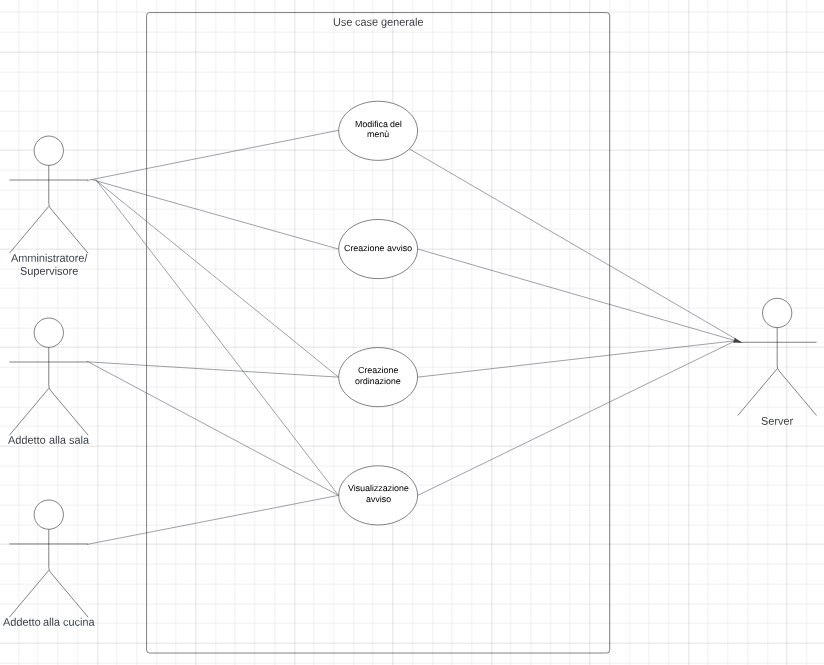
\includegraphics[scale=0.8]{img/use_case/use_case_generale.png}
\end{center}

\subsubsection{Creazione piatto}
La creazione del piatto è una delle funzionalità più elaborate, in quanto, non basterà essere un amministratore/supervisore e inserire i dati (nome, descrizione, allergeni, categoria e prezzo) necessari alla creazione di un piatto. Verrà infatti controllata l'esistenza del piatto e, nel caso di esito positivo il piatto non verrà creato, altrimenti verrà aggiunto alla categoria selezionata.
\begin{center}
  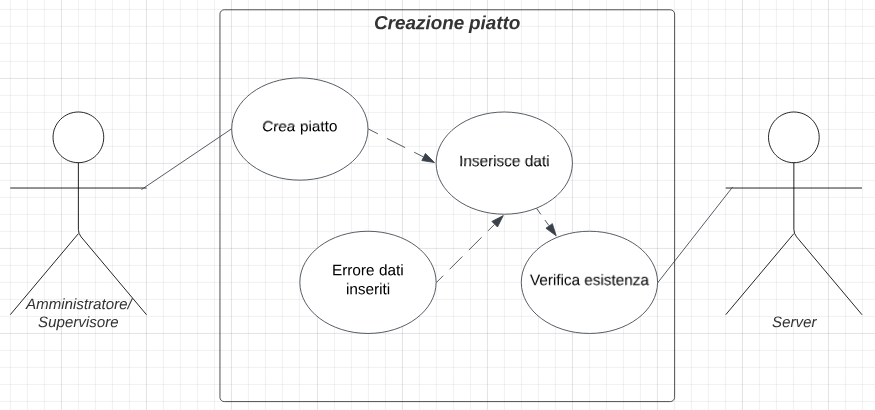
\includegraphics[scale=0.65]{img/use_case/use_case-creazione_piatto.png}
\end{center}
\subsubsection{Eliminazione piatto}
L'eliminazione del piatto è tutto sommato una funzionalità semplice ed autoesplicativa. Viene semplicemente scelto, da un amministratore/supervisore, il piatto che si desidera eliminare, una volta eliminato ci sarà una richiesta di conferma di eliminazione.
\begin{center}
  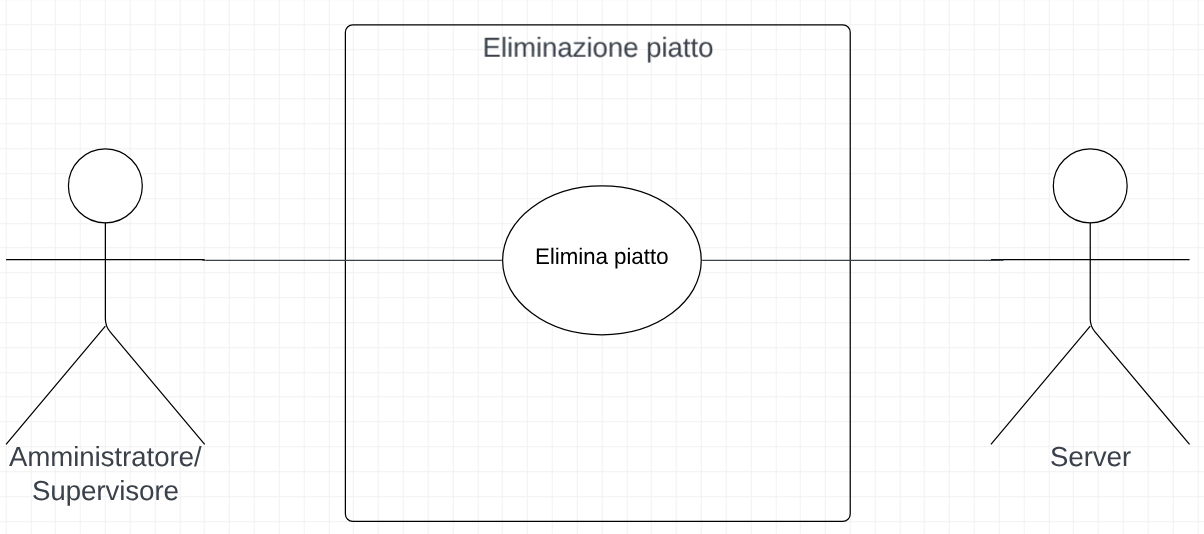
\includegraphics[scale=0.5]{img/use_case/use_case-eliminazione_piatto.png}
\end{center}
\newpage
\subsubsection{Creazione ordinazione}
La creazione di un ordinazione è un requistio fondamentale per la corretta gestione di un'attività di ristorazione che sia essa una tavola calda, un Autogrill o un classico risotrante. Per prima cosa è necessario che l'utente registrato che prova a creare un ordinazione è un "addetto alla sala". Infatti nel caso in cui l'utente registrato non appartiene a questa categoria, non gli sarà permesso a priori la creazione di un ordinazione. Per creare un ordinazione è necessario scegliere un tavolo (tramite l'identificativo associato), e selezionare i piatti che si vogliono aggiungere all'ordinazione (sarà possibile registrare più ordinazioni per lo stesso tavolo in momenti separati).
\begin{center}
  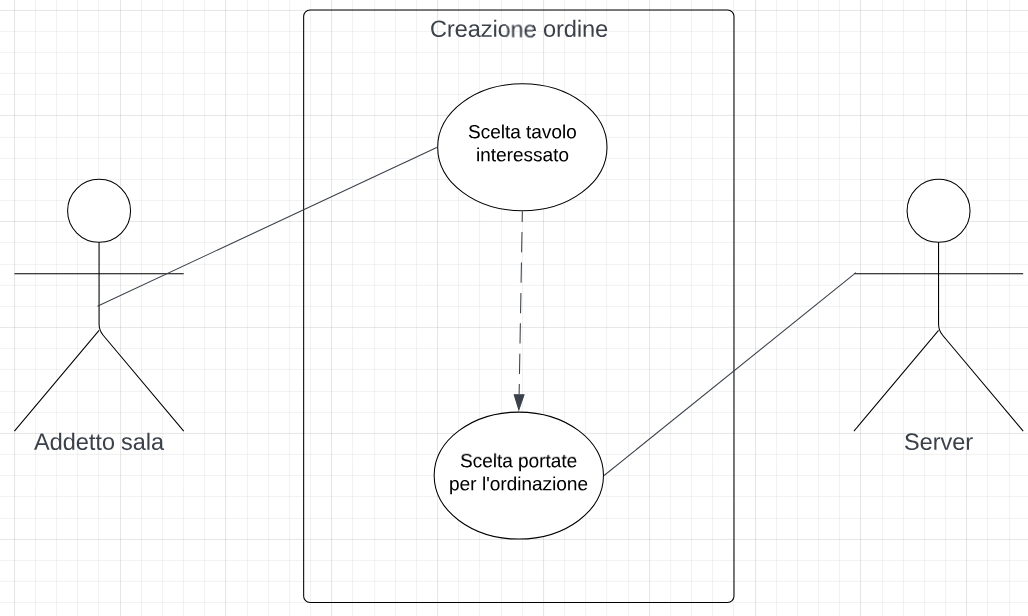
\includegraphics[scale=0.6]{img/use_case/use_case-creazione_ordine.png}
\end{center}
\newpage
\subsubsection{Creazione notifica}
La creazione di un avviso (notifica), è un aspetto fondamentale del software in quanto permette all'amministratore/supervisore di comunicare informazioni importanti indistintamente ad ogni utente. Infatti gli unici utenti con permessi per creare un avviso (notifica) sono proprio l'amministratore e i supervisori.
\begin{center}
  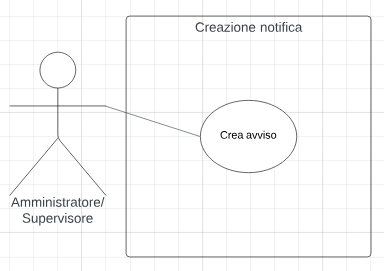
\includegraphics[scale=0.6]{img/use_case/use_case-creazione_notifica.png}
\end{center}
\newpage
\subsection{Tabelle cockburn}
Ci è stato richiesto di presentare, tra i casi d'uso assegnati, quattro casi
specifici a scelta descrivendoli tramite \textbf{tabelle di Cockburn}.
\paragraph{Cosa sono?} Le tabelle di Cockburn (create da \textit{Alistair Cockburn}, dal quale prendono il nome) sono un formalismo di rappresentazione dei casi d'uso.\\
Sono la rappresentazione di un main scenario (nel nostro primo caso la creazione di un'ordinazione) nel quale uno o più attori interagiscono
tra loro attraverso l'invocazione di trigger e descrivendo (in formato tabellare) gli eventi.
\\
\\Per garantire una certa corenza al committente e una comprensione a tutto tondo abbiamo scelto gli stessi casi esplorati nella presentazione dei casi d'uso.
\subsubsection{Creazione ordinazione}

\begin{table}[H]
  \def\arraystretch{1.5}
  \begin{tabularx}{\linewidth}{|l|X|X|X|}
    \hline Use Case \#1                      & \multicolumn{3} {l|}{Creazione ordinazione}                                                                                                                                                         \\ \hline Goal in
    Context                                  & \multicolumn{3}{>{\hsize=\dimexpr 3\hsize+4\tabcolsep+2\arrayrulewidth\relax}X|}{Si vuole creare una nuova ordinazione}                                                                             \\
    \hline Preconditions                     &
    \multicolumn{3}{l|}{L'utente deve essere autenticato correttamente ed in \textbf{M2}}                                                                                                                                                          \\
    \hline Success End Conditions            &
    \multicolumn{3}{l|}{L'ordinazione è stata creata}                                                                                                                                                                                              \\
    \hline Failed End Conditions             &
    \multicolumn{3}{l|}{L'ordinazione non è stata creata}                                                                                                                                                                                          \\
    \hline Primary Actor                     &
    \multicolumn{3}{l|}{Utente autenticato}                                                                                                                                                                                                        \\
    \hline Trigger                           & \multicolumn{3}{l|}{L'utente autenticato preme il tasto "crea ordinazione"}                                                                                                                         \\

    \hline \multirow{2}{*}{Description}      & Step                                                                                                                    & Utente autenticato             & Sistema                                  \\
    \cline{2-4}                              & 1                                                                                                                       & Preme "Aggiungi ordinazione"   &                                          \\
    \cline{2-4}                              & 2                                                                                                                       &                                & Mostra M3                                \\
    \cline{2-4}                              & 3                                                                                                                       & Seleziona i piatti da inserire &                                          \\
    \cline{2-4}                              & 4                                                                                                                       & Conferma l'ordine              &                                          \\
    \cline{2-4}                              & 5                                                                                                                       &                                & Chiude M3                                \\
    \cline{2-4}                              & 6                                                                                                                       &                                & Mostra messaggio di successo             \\
    \hline \multirow{2}{*}{Extensions\#1: }  & Step                                                                                                                    & Utente autenticato             & Sistema                                  \\
    \cline{2-4}Categoria o piatto non validi & 6.1                                                                                                                     &                                & Mostra messaggio d'errore                \\
    \hline \multirow{2}{*}{Extensions\#2: }  & Step                                                                                                                    & Utente autenticato             & Sistema                                  \\
    \cline{2-4} Impossibile connettersi      & 6.2                                                                                                                     &                                & Mostra messaggio "Errore di connessione" \\
    \hline
  \end{tabularx}
\end{table}
\subsubsection{Eliminazione piatto}
\begin{table}[H]
  \def\arraystretch{1.5}
  \begin{tabularx}{\linewidth}{|l|X|X|X|}
    \hline Use Case \#2                     & \multicolumn{3} {l|}{Eliminazione piatto}                                                                                                                                                     \\ \hline Goal in
    Context                                 & \multicolumn{3}{>{\hsize=\dimexpr 3\hsize+4\tabcolsep+2\arrayrulewidth\relax}X|}{L'utente vuole eliminare un piatto dal menù}                                                                 \\
    \hline Preconditions                    &
    \multicolumn{3}{l|}{L'utente deve essere autenticato correttamente ed in \textbf{M4}}                                                                                                                                                   \\
    \hline Success End Conditions           &
    \multicolumn{3}{l|}{Il piatto è stato eliminato}                                                                                                                                                                                        \\
    \hline Failed End Conditions            &
    \multicolumn{3}{l|}{Il piatto non è stato eliminato}                                                                                                                                                                                    \\
    \hline Primary Actor                    &
    \multicolumn{3}{l|}{Utente autenticato}                                                                                                                                                                                                 \\
    \hline Trigger                          & \multicolumn{3}{l|}{L'utente autenticato preme il tasto "elimina" sul piatto desiderato}                                                                                                      \\

    \hline \multirow{2}{*}{Description}     & Step                                                                                                                          & Utente autenticato & Sistema                                  \\
    \cline{2-4}                             & 1                                                                                                                             &                    & Mostra M5                                \\
    \cline{2-4}                             & 2                                                                                                                             & Clicca "ELIMINA"   &                                          \\
    \cline{2-4}                             & 3                                                                                                                             &                    & chiude M5                                \\
    \cline{2-4}                             & 4                                                                                                                             &                    & Mostra messaggio di successo             \\
    \hline \multirow{2}{*}{Extensions\#1: } & Step                                                                                                                          & Utente autenticato & Sistema                                  \\
    \cline{2-4}L'utente clicca "INDIETRO"   & 2.1                                                                                                                           & Clicca "INDIETRO"  &                                          \\
    \cline{2-4}                             & 3.1                                                                                                                           &                    & Chiude M5                                \\
    \hline \multirow{2}{*}{Extensions\#2: } & Step                                                                                                                          & Utente autenticato & Sistema                                  \\
    \cline{2-4} Impossibile connettersi     & 4.2                                                                                                                           &                    & Mostra messaggio "Errore di connessione" \\
    \hline
  \end{tabularx}
\end{table}

\subsubsection{Creazione piatto}
\begin{table}[H]
  \def\arraystretch{1.5}
  \begin{tabularx}{\linewidth}{|l|X|X|X|}
    \hline Use Case \#3                     & \multicolumn{3} {l|}{Creazione piatto}                                                                                                                                               \\ \hline Goal in
    Context                                 & \multicolumn{3}{>{\hsize=\dimexpr 3\hsize+4\tabcolsep+2\arrayrulewidth\relax}X|}{L'utente vuole creare un piatto}                                                                    \\
    \hline Preconditions                    &
    \multicolumn{3}{l|}{L'utente deve essere autenticato correttamente ed in \textbf{M6}}                                                                                                                                          \\
    \hline Success End Conditions           &
    \multicolumn{3}{l|}{Il piatto è stato creato}                                                                                                                                                                                  \\
    \hline Failed End Conditions            &
    \multicolumn{3}{l|}{Il piatto non è stato creato}                                                                                                                                                                              \\
    \hline Primary Actor                    &
    \multicolumn{3}{l|}{Utente autenticato}                                                                                                                                                                                        \\
    \hline Trigger                          & \multicolumn{3}{l|}{L'utente autenticato preme il tasto "crea piatto" in \textbf{M6}}                                                                                                \\

    \hline \multirow{2}{*}{Description}     & Step                                                                                                              & Utente autenticato    & Sistema                                  \\
    \cline{2-4}                             & 1                                                                                                                 & Clicca "crea piatto"  &                                          \\
    \cline{2-4}                             & 2                                                                                                                 &                       & chiude M7                                \\
    \cline{2-4}                             & 3                                                                                                                 & Riempie i campi       &                                          \\
    \cline{2-4}                             & 4                                                                                                                 & Conferma la creazione &                                          \\
    \cline{2-4}                             & 5                                                                                                                 &                       & Chiude M7                                \\
    \cline{2-4}                             & 6                                                                                                                 &                       & Mostra messaggio di successo             \\
    \hline \multirow{2}{*}{Extensions\#1: } & Step                                                                                                              & Utente autenticato    & Sistema                                  \\
    \cline{2-4} campi non validi            & 5.1                                                                                                               &                       & Svuota i campi inseriti                  \\
    \cline{2-4}                             & 6.1                                                                                                               &                       & Mostra messaggio d'errore                \\
    \hline \multirow{2}{*}{Extensions\#2: } & Step                                                                                                              & Utente autenticato    & Sistema                                  \\
    \cline{2-4} Uno o più campi vuoti       & 5.2                                                                                                               &                       & Svuota i campi inseriti                  \\
    \cline{2-4}                             & 6.2                                                                                                               &                       & Mostra messaggio d'errore                \\

    \hline \multirow{2}{*}{Extensions\#3: } & Step                                                                                                              & Utente autenticato    & Sistema                                  \\
    \cline{2-4} Impossibile connettersi     & 5.3                                                                                                               &                       & Mostra messaggio "Errore di connessione" \\
    \hline
  \end{tabularx}
\end{table}
\subsubsection{Creazione notifica}
\begin{table}[H]
  \def\arraystretch{1.5}
  \begin{tabularx}{\linewidth}{|l|X|X|X|}
    \hline Use Case \#4                     & \multicolumn{3} {l|}{Creazione notifica}                                                                                                                                                 \\ \hline Goal in
    Context                                 & \multicolumn{3}{>{\hsize=\dimexpr 3\hsize+4\tabcolsep+2\arrayrulewidth\relax}X|}{L'utente vuole creare una notifica}                                                                     \\
    \hline Preconditions                    &
    \multicolumn{3}{l|}{L'utente deve essere autenticato correttamente ed in \textbf{M8}}                                                                                                                                              \\
    \hline Success End Conditions           &
    \multicolumn{3}{l|}{La notifica è stata creata}                                                                                                                                                                                    \\
    \hline Failed End Conditions            &
    \multicolumn{3}{l|}{La notifica non è stata creata}                                                                                                                                                                                \\
    \hline Primary Actor                    &
    \multicolumn{3}{l|}{Utente autenticato}                                                                                                                                                                                            \\
    \hline Trigger                          & \multicolumn{3}{l|}{L'utente autenticato preme il tasto "crea notifica" in \textbf{M8}}                                                                                                  \\

    \hline \multirow{2}{*}{Description}     & Step                                                                                                                 & Utente autenticato     & Sistema                                  \\
    \cline{2-4}                             & 1                                                                                                                    & Clicca "crea notifica" &                                          \\
    \cline{2-4}                             & 2                                                                                                                    &                        & chiude M9                                \\
    \cline{2-4}                             & 3                                                                                                                    & Riempie i campi        &                                          \\
    \cline{2-4}                             & 4                                                                                                                    & Conferma la creazione  &                                          \\
    \cline{2-4}                             & 5                                                                                                                    &                        & Chiude M9                                \\
    \cline{2-4}                             & 6                                                                                                                    &                        & Mostra messaggio di successo             \\
    \hline \multirow{2}{*}{Extensions\#1: } & Step                                                                                                                 & Utente autenticato     & Sistema                                  \\
    \cline{2-4} Uno o più campi vuoti       & 5.2                                                                                                                  &                        & Svuota i campi inseriti                  \\
    \cline{2-4}                             & 5.1                                                                                                                  &                        & Mostra messaggio d'errore                \\

    \hline \multirow{2}{*}{Extensions\#2: } & Step                                                                                                                 & Utente autenticato     & Sistema                                  \\
    \cline{2-4} Impossibile connettersi     & 5.2                                                                                                                  &                        & Mostra messaggio "Errore di connessione" \\
    \hline
  \end{tabularx}
\end{table}

\newpage
\subsection{Mock-Up}
Un mock-up , è una realizzazione a scopo illustrativo o meramente espositivo, di un oggetto o un sistema, senza le complete funzioni
dell'originale; un mockup può rappresentare la totalità o solo una parte dell'originale di riferimento (già esistente o in fase di progetto), essere in scala
reale oppure variata.
\begin{center}
  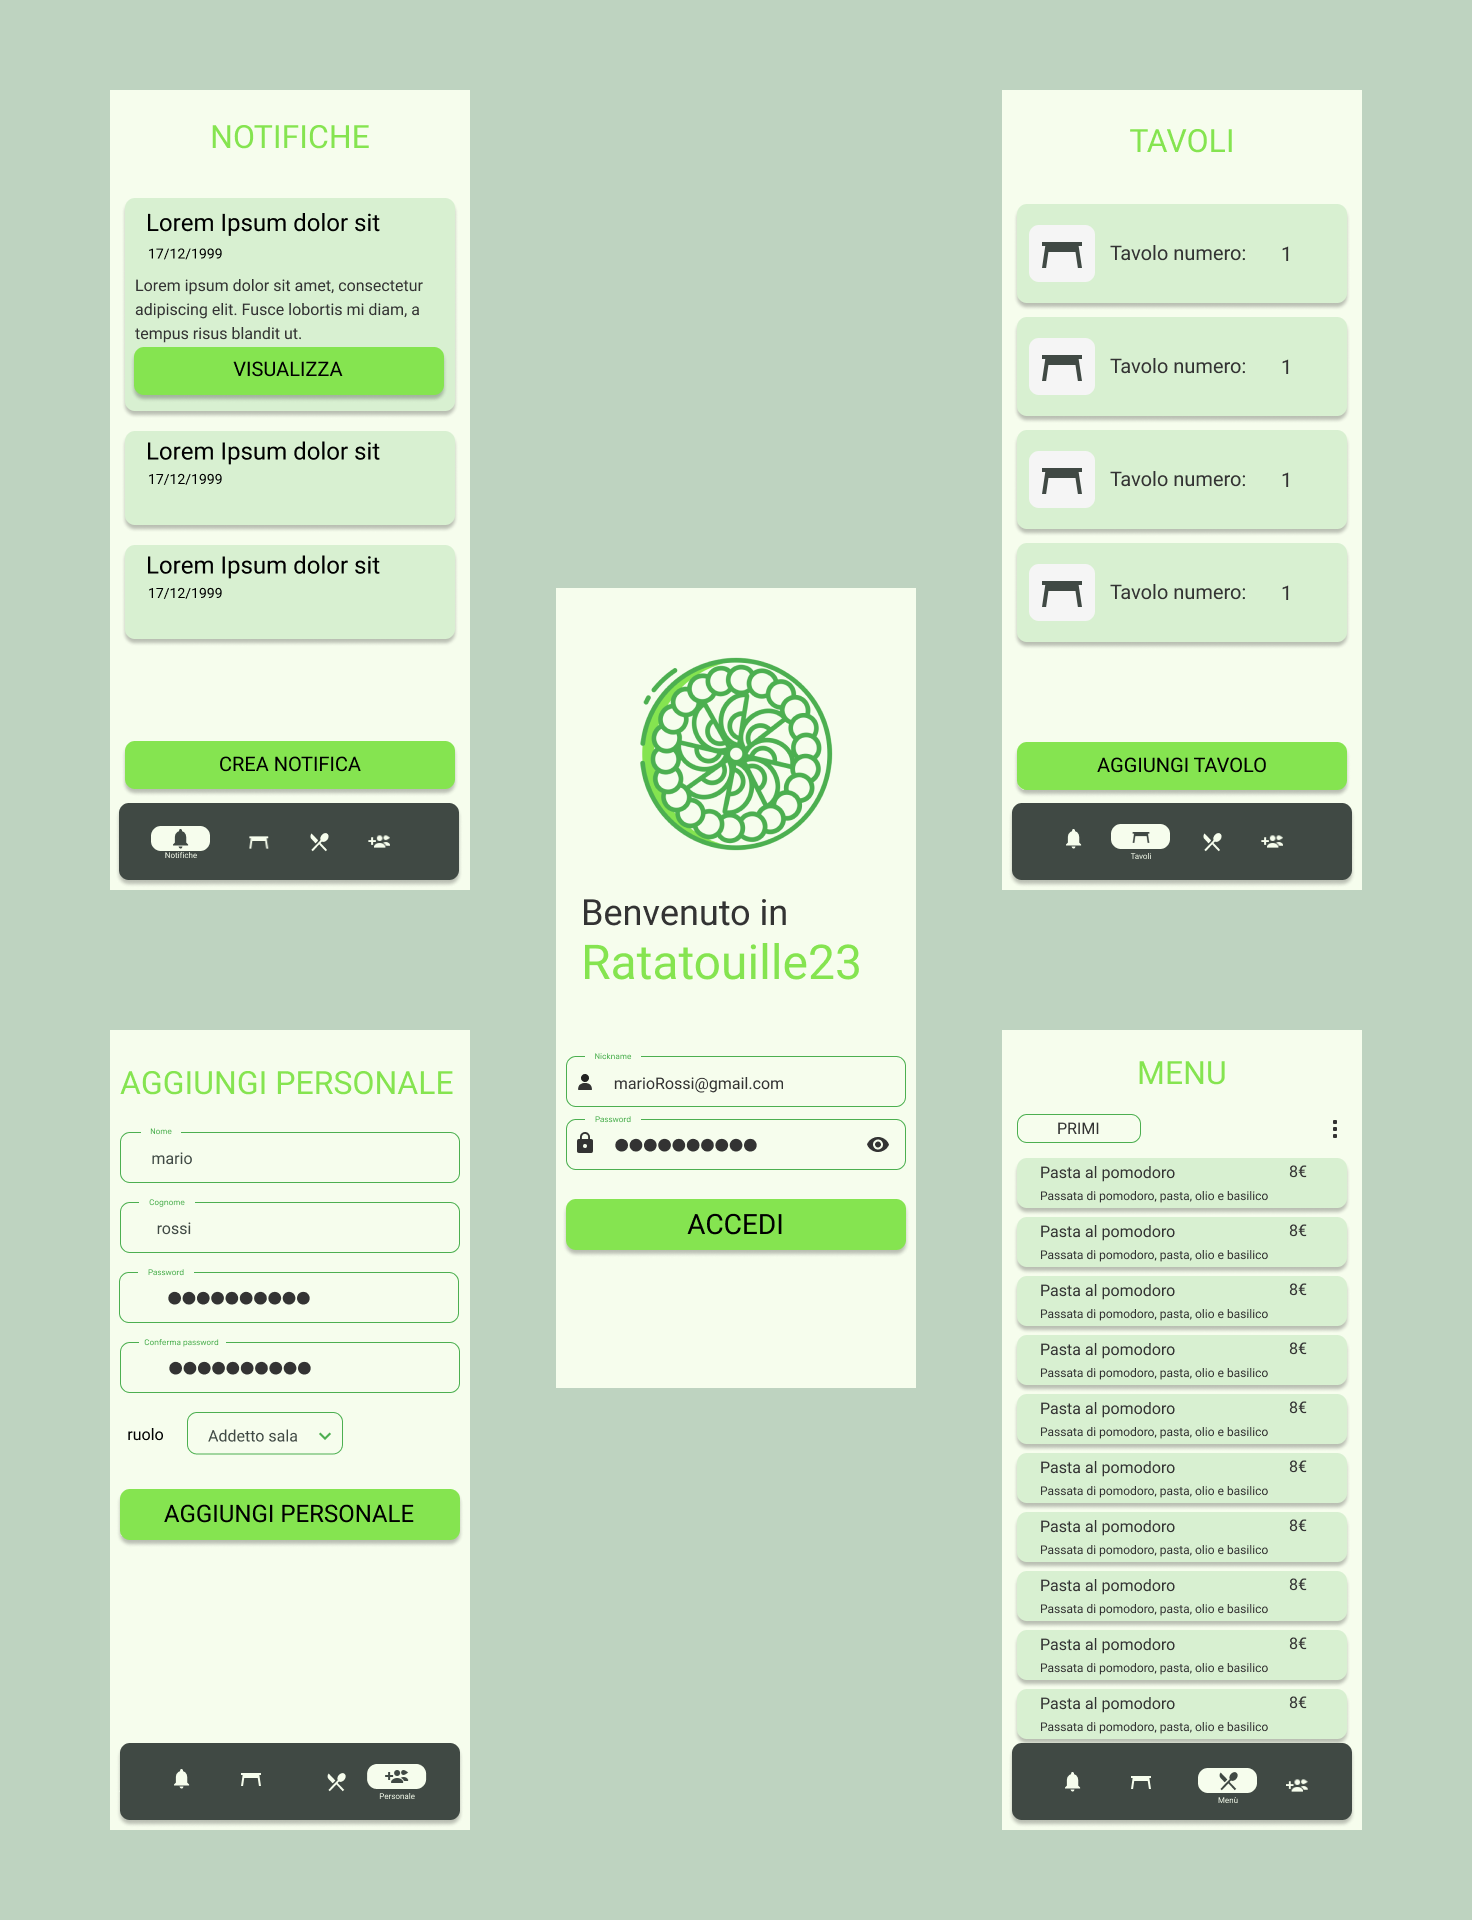
\includegraphics[scale=0.2]{img/Mock-up.doc}
\end{center}
La versione del mock-up qui sopra rappresenta le schermate principali dell'applicazione. Nella realizzazione di quest'applicazione c'è stato uno studio del colore e dell'usabilità, con una palette creata appositamente per non stancare gli occhi e rendere il tutto più "vicino" al cibo possibile.\\
Di seguito andremo a visualizzare i mock-up dei metodi scelti dal team.
\newpage
\subsubsection{Creazione ordinazione}
Questa schermata rappresenta l'elenco dei tavoli già presenti nel database, quando verrà selezionato un tavolo premendoci sopra, il sistema aprirà \textbf{M2}.
\begin{figure}[H]
  \centering
  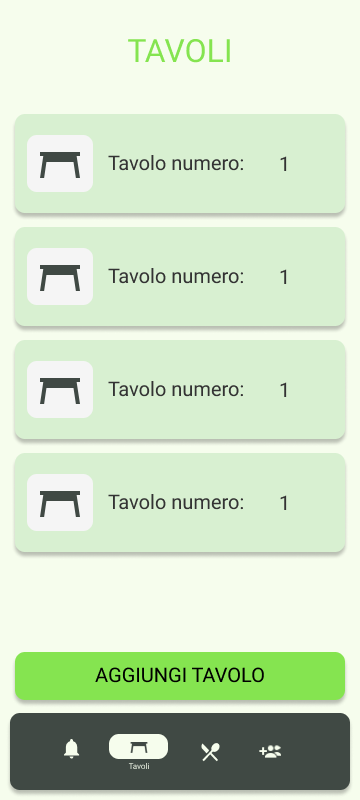
\includegraphics[scale=0.6]{img/mock-up/tables.png}
  \caption{pagina dei tavoli}
\end{figure}\newpage
\begin{figure}[H]
  Una volta aperta \textbf{M2} ci verrà presentato l'elenco delle portate del tavolo selezionato (nel nostro caso, il tavolo 1). Quando l'utente cliccherà il pulsante "Aggiungi ordinazione" il sistema aprirà \textbf{M3}.
  \centering
  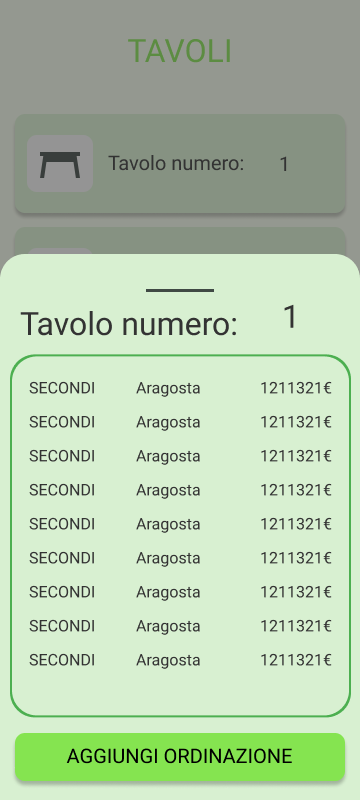
\includegraphics[scale=0.6]{img/mock-up/Table_content.png}
  \caption{Contenuto del tavolo n°1.}
\end{figure}\newpage
Ora che ci troviamo in \textbf{M3} potremo usare i due spinner (categoria e piatto) per selezionare il piatto che desideriamo aggiungere all'ordinazione e quando saremo soddisfatti potremo confermarlo.
\begin{figure}[H]
  \centering
  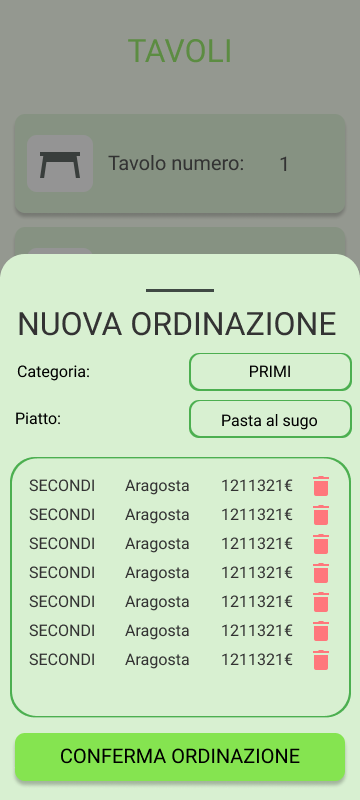
\includegraphics[scale=0.6]{img/mock-up/New_order.png}
  \caption{Nuova ordinazione per il tavolo n°1.}
\end{figure}
\newpage
\subsubsection{Eliminazione piatto}
La schermata riportata qui sotto mostra il menù del ristorante con la possibilità di eliminare i piatti da esso. Qualora l'utente dovesse cliccare "ELIMINA" su uno dei piatti si aprirà \textbf{M5}.
\begin{figure}[H]
  \centering
  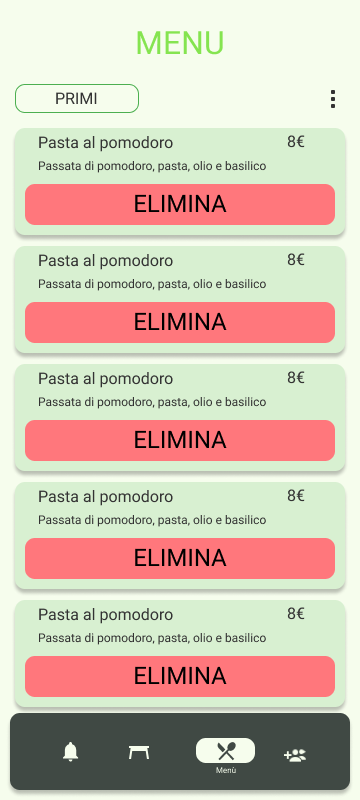
\includegraphics[scale=0.6]{img/mock-up/Dish_deletion.png}
  \caption{Menù ristorante con piatti da eliminare.}
\end{figure}
\newpage
In questa schermata l'utente potrà confermare l'eliminazione del piatto oppure tornare indietro, annullando così l'eliminazione.
\begin{figure}[H]
  \centering
  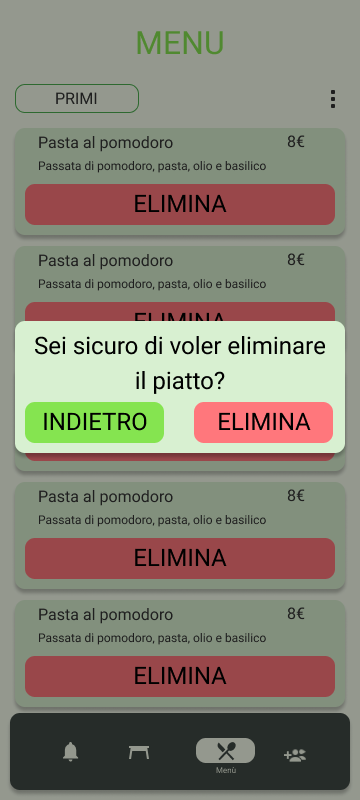
\includegraphics[scale=0.6]{img/mock-up/Confirm_dish_deletion.png}
  \caption{Conferma eliminazione piatto.}
\end{figure}
\newpage
\subsubsection{Creazione piatto}
La creazione del piatto è una delle funzionalità più importanti, infatti è quella che ci permette di popolare il menù con piatti creati da noi. Per creare un piatto, bisognerà che l'utente di trovi nella schermata del menù (\textbf{M6}).
\begin{figure}[H]
  \centering
  \includegraphics[scale=0.6]{img/mock-up/Menù.png}
  \caption{Schermata del menù.}
\end{figure}
\newpage
In questa scermata, tramite i tre puntini in alto a destra, possiamo attivare la funzione di creazione di un piatto, che ci aprirà \textbf{M7}.
\begin{figure}[H]
  \centering
  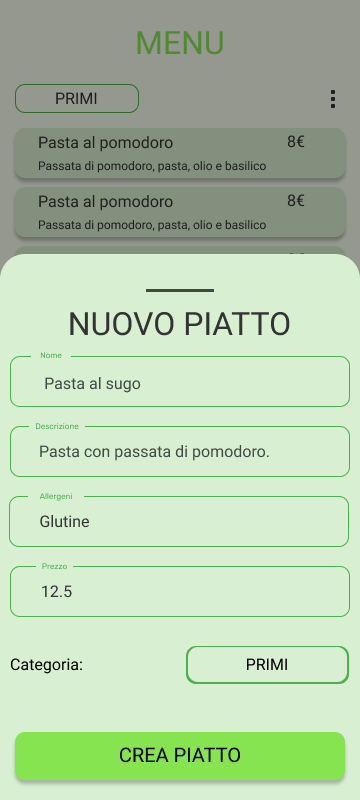
\includegraphics[scale=0.6]{img/mock-up/create_dish.png}
  \caption{Schermata del menù.}
\end{figure}
Una volta in questa schermata non bisognerà fare altro che riempire i campi necessari e confermare la craezione.
\newpage
\subsubsection{Creazione notifica}
La creazione di una notifica, permette ad un amministratore/supervisore, di mandare un messaggio a tutti i suoi dipendente, così da poter comunicare avvisi importanti indistintamente ad ogni dipendente qualora si voglia. Per farlo, l'utente deve trovarsi in \textbf{M8} ($\downarrow$) e premere "CREA NOTIFICA".
\begin{figure}[H]
  \centering
  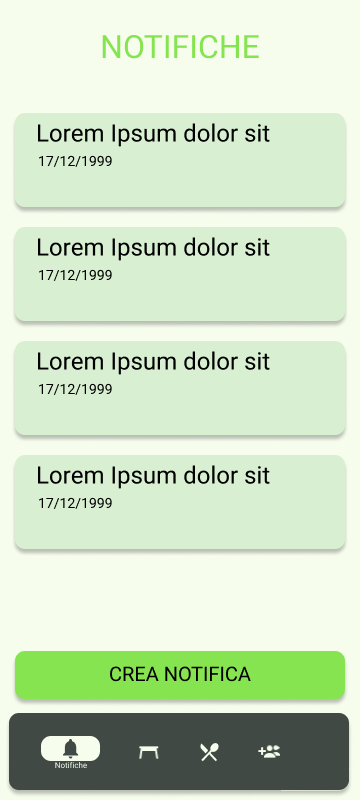
\includegraphics[scale=0.6]{img/mock-up/Notificaitons.png}
  \caption{Schermata delle notifiche.}
\end{figure}
\newpage
Una volta premuto "CREA NOTIFICA", il sistema mostrerà \textbf{M9} ($\downarrow$), al cui interno ci saranno due campi richiesti (titolo e testo, la data verrà prelevata in automatico dal sistema), una volta compilati, l'utente può premere "CREA NOTIFICA".
\begin{figure}[H]
  \centering
  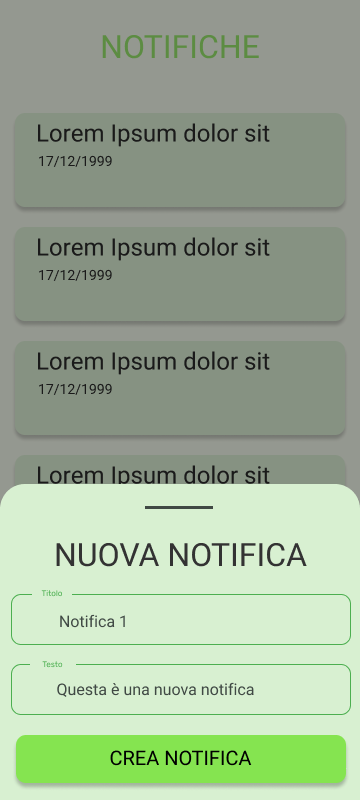
\includegraphics[scale=0.6]{img/mock-up/create_notifications.png}
  \caption{Schermata per la creazione di una notifica.}
\end{figure}
\newpage
\subsection{Individuazione del target a priori}
Ratatouille23\texttrademark \ nasce con l'idea di creare un sistema efficiente e affidabile per la gestione di attività di ristorazione. Nello specifico poter permettere ad un responsabile di poter dividere dettagliatamente le mansioni di un dipendente con la possibilità di assumere dei collaboratori (e.g. supervisore).
Il target che si può definire da una prima analisi delle funzionalità e casi d'uso, è il seguente:
\begin{itemize}
  \item Camerieri e manager di ristorante.
  \item Cuochi, sous chef e aiuto cuoco.
  \item Proprietario e dirigente di ristorante.
\end{itemize}
Questa prima analisi può fornirci una visione sommaria delle personas.
\subsubsection{Personas}
Il focus principale per noi è stato quello di analizzare 2 aspetti che abbiamo ritenuto fondamentali
per individuare le user personas così da poter sviluppare un software cucito su misura:
\begin{enumerate}
  \item \textbf{Età:} la fascia d'età che abbiamo potuto notare essere più conforme all'utente ideale è quella dei 18-65 anni, in modo da comprendere uno studente ma anche un cuoco di fama mondiale con alle spalle numerosi anni di esperienza.
  \item \textbf{Background:} per background s'intende la formazione dell'utente. Infatti un nostro utente può essere uno studente, che lavora il weekend per poter pagare l'affitto da fuorisede, così come può essere un ragazzo con formazione \textit{sommelier} o una ragazza che ha conseguito un corso all'\textit{ALMA}.
\end{enumerate}
Questo ci permette di pianificare sviluppi futuri del nostro software. Potremmo infatti creare una sezione dedicata ai vini, facendo in modo che il sommelier consigli in base ai piatti ordinati, quali vini si accostano meglio.\\
Potremmo aggiungere una sezione con dei percorsi culinari, studiati in precedenza da un personale esperto e preparato. Così facendo potremo fidelizzare i nostri utenti dandogli completa libertà per la gestione della loro attività.
\newpage
\paragraph{Lucia Zhang}
La prima user persona è stata utilizzata per raccoglire il target di utenti nella fascia compresa tra i 25-35 anni, che hanno un'alta competenza con la tecnologia e che sono già avviati, nel mondo del lavoro.
\renewcommand{\figurename}{}
\renewcommand{\thefigure}{Fig.\arabic{figure}}
\setcounter{figure}{\getrefnumber{1}}
\begin{figure}[H]
  \centering
  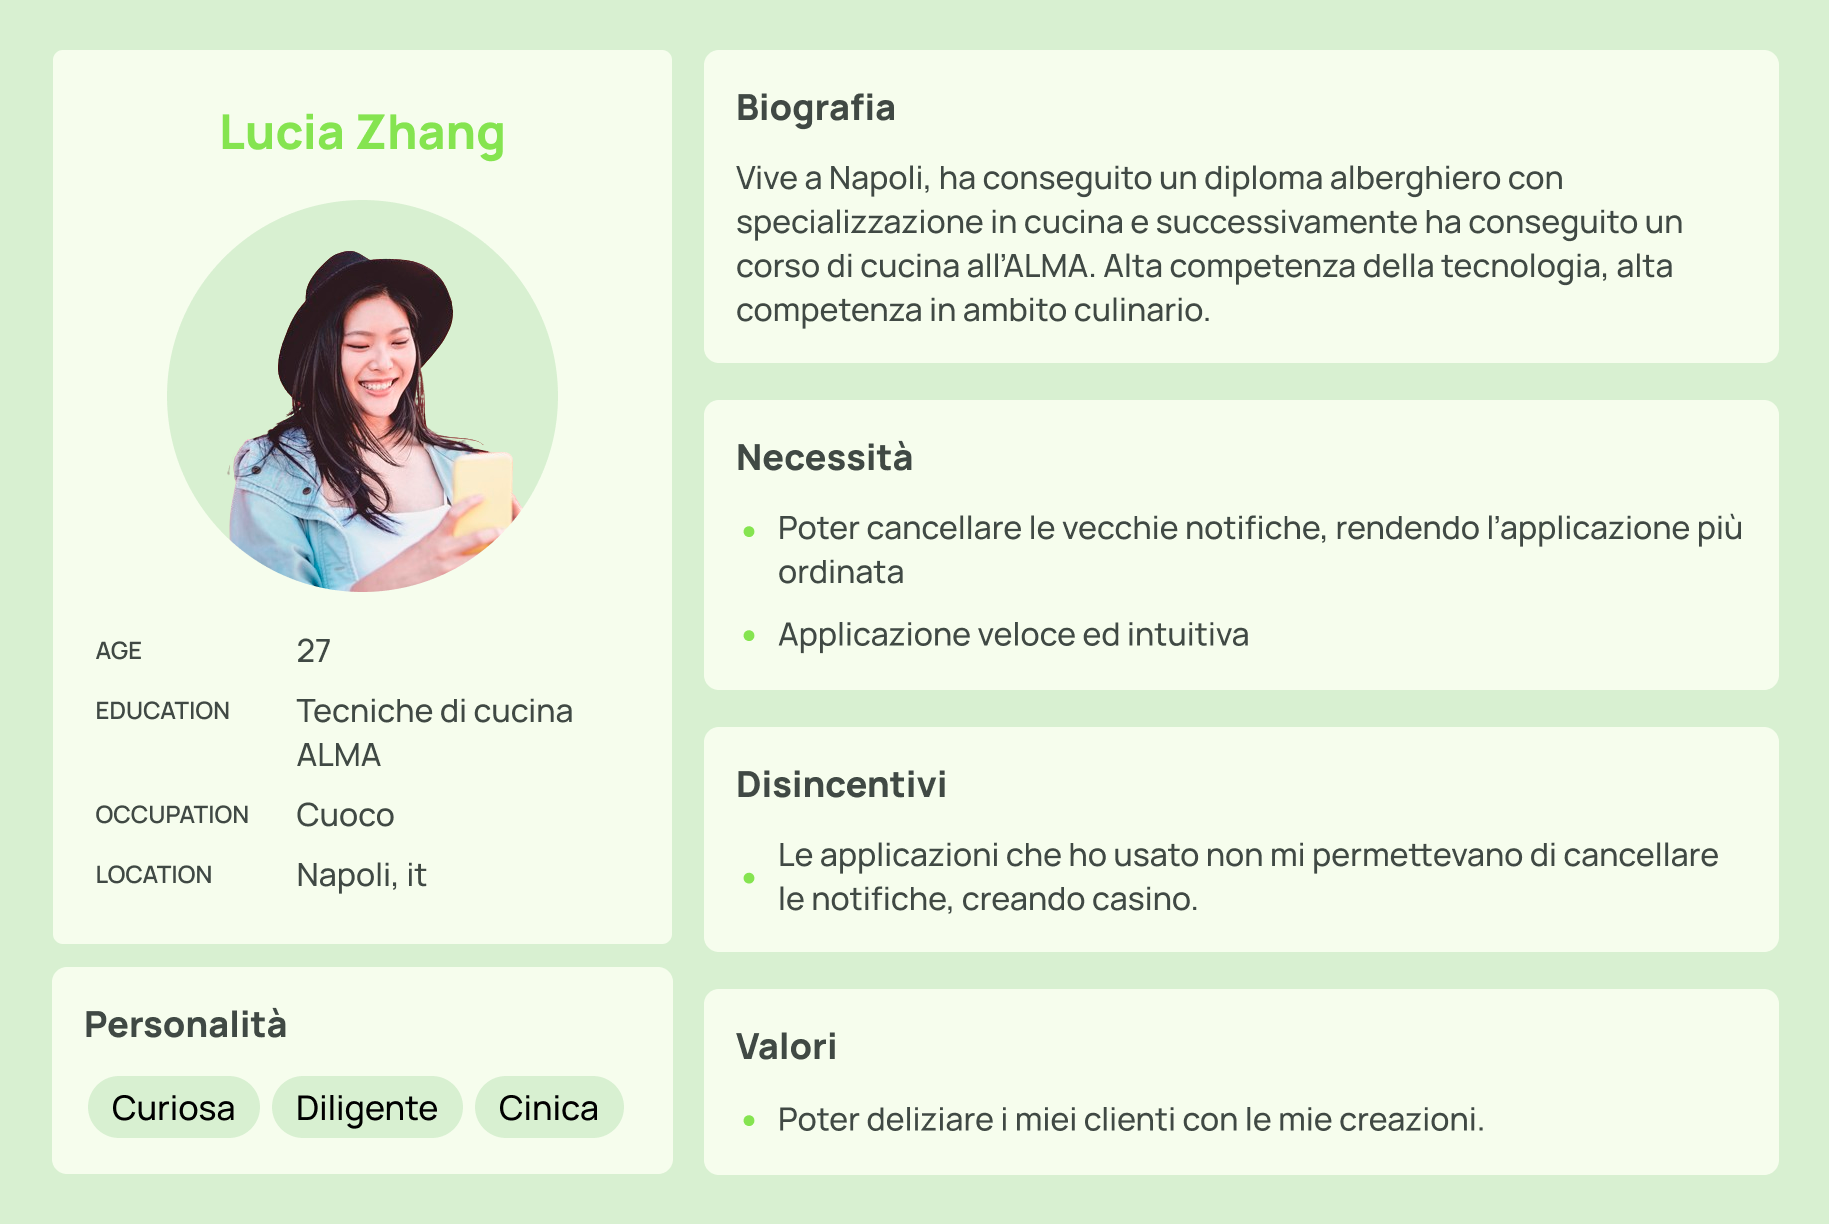
\includegraphics[scale=0.25]{img/personas/Lucia_zhang_persona.png}
  \caption{User persona n.1.}
\end{figure}

\newpage
\paragraph{Stefano Iamunno}
La seconda user persona è stata utilizzata per raccoglire il target di utenti nella fascia d'età compresa tra i 18-25 anni, che hanno un'alta competenza tecnologica ma che si sono appena approcciati al mondo del lavoro.
\begin{figure}[H]
  \centering
  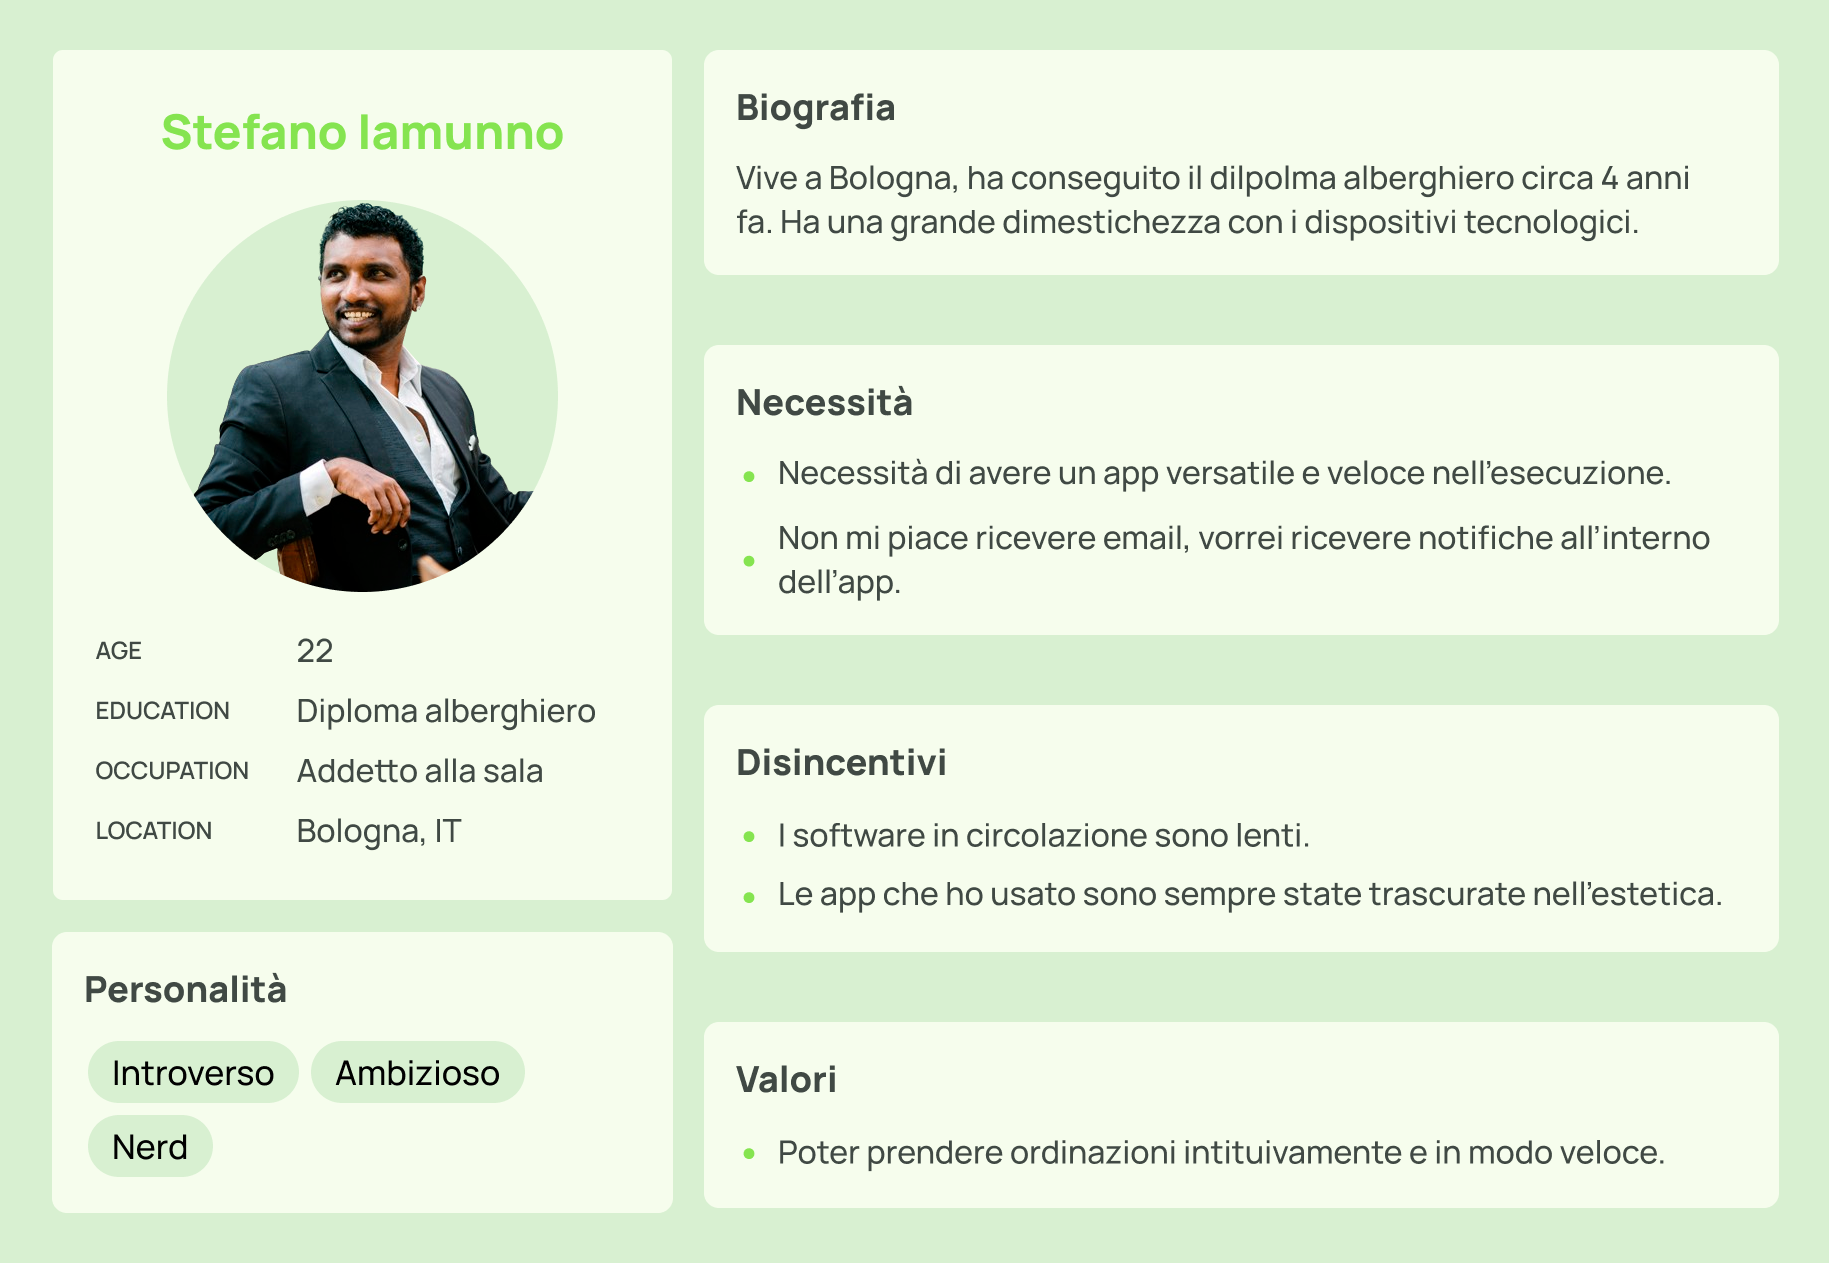
\includegraphics[scale=0.25]{img/personas/Stefano_iamunno_persona.png}
  \caption{User persona n.2.}
\end{figure}
\newpage
\paragraph{Maria colombo}
La terza user persona è stata utilizzata per raccoglire il target di utenti nella fascia d'età compresa tra i 35-65 anni, che hanno una bassa competenza tecnologica ma con una vasta esperienza nel mondo del lavoro. Sono utenti che con la loro esperienza lavorativa possono assumere pressochè qualsiasi ruolo all'interno di un'attività di ristorazione.

\begin{figure}[H]
  \centering
  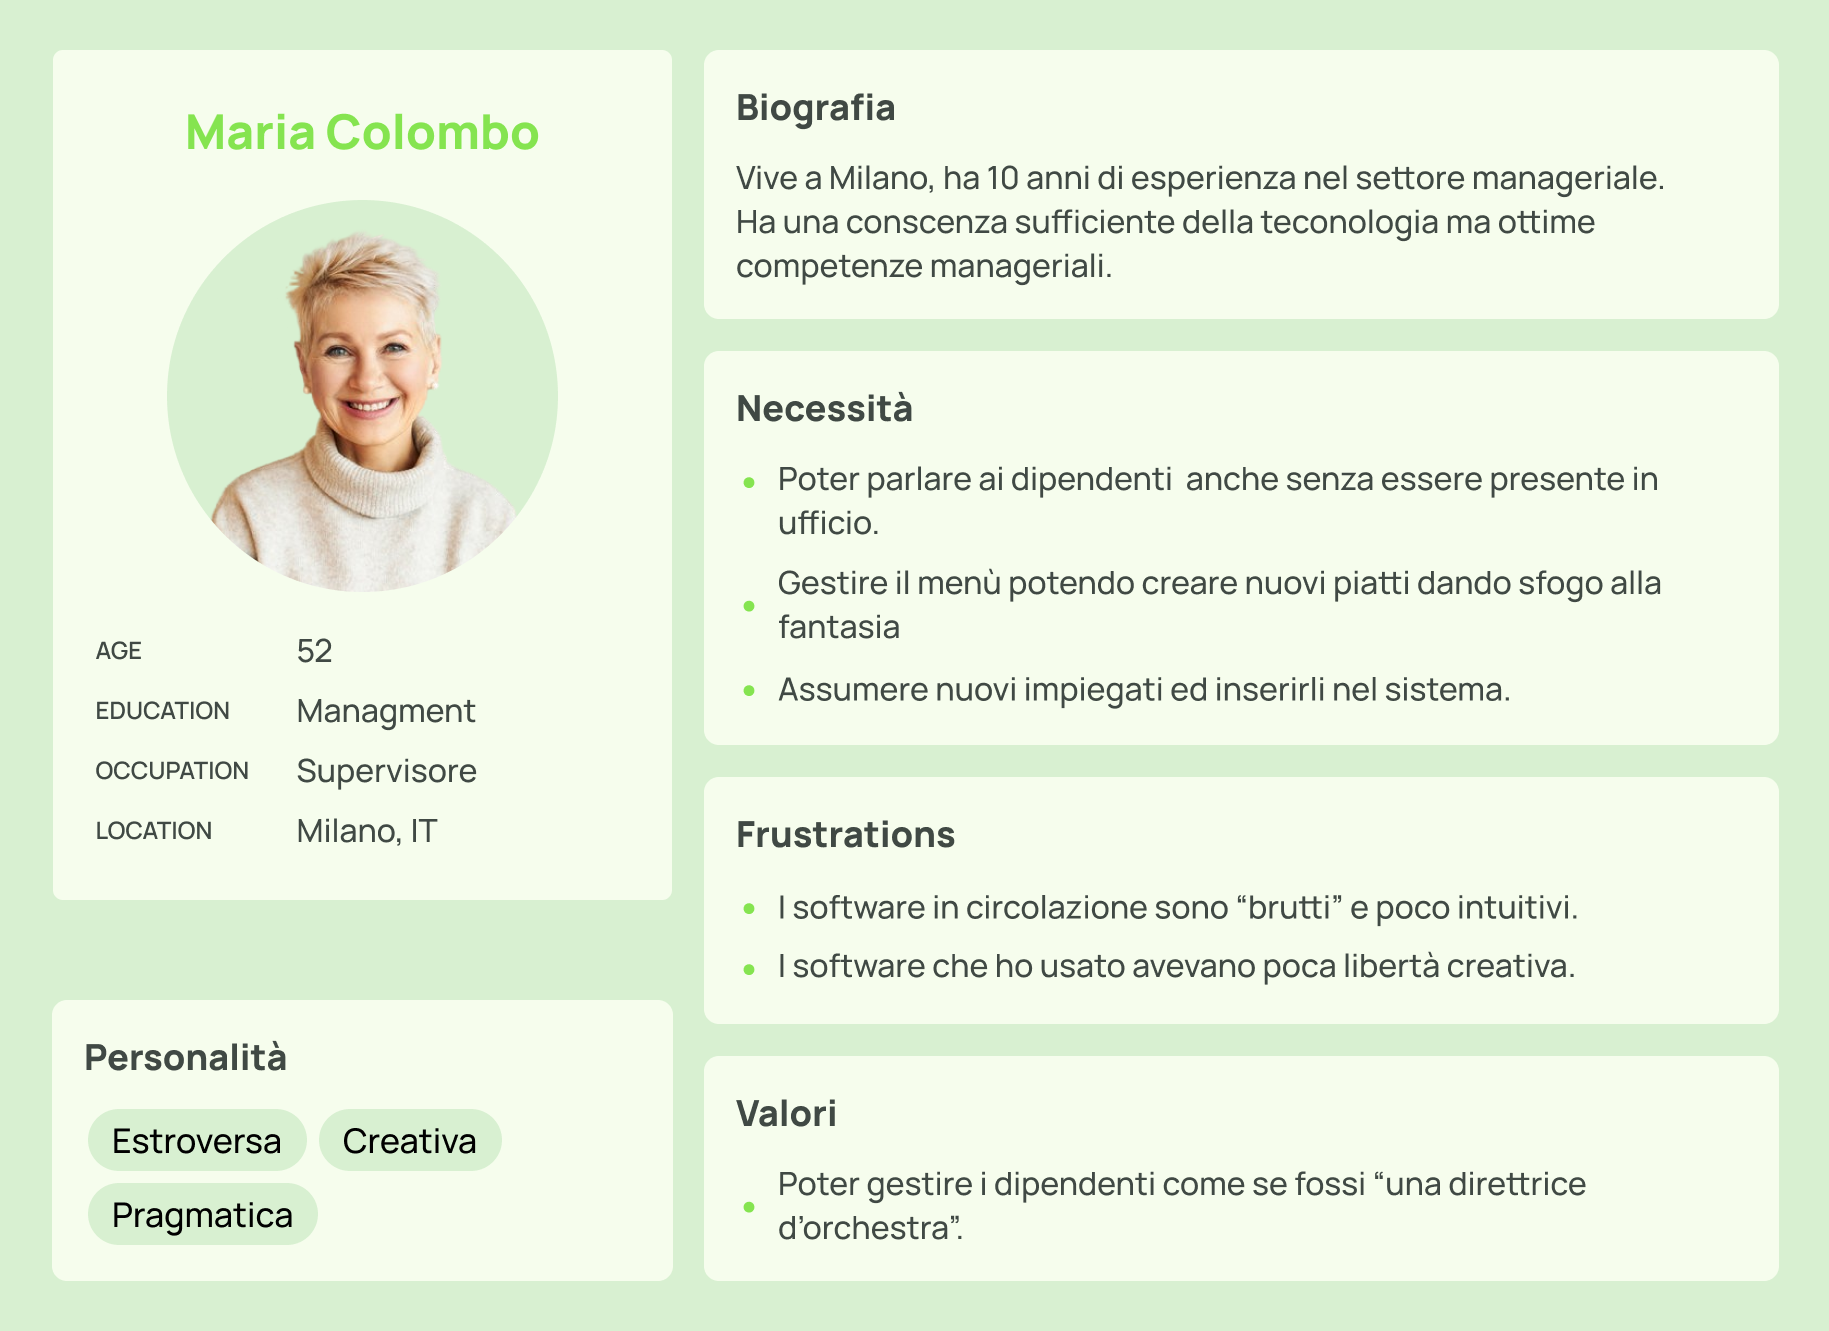
\includegraphics[scale=0.25]{img/personas/Maria_colombo_persona.png}
  \caption{User persona n.3.}
\end{figure}\newpage
\subsection{Valutazione dell'usabilità a priori}
\begin{quote}
  L'usabilità di un prodotto è il grado con cui esso può essere usato da specificati utenti per raggiungere specificati obiettivi con efficacia, efficienza e soddisfazione in uno specificato contesto d'uso.
\end{quote}
Facendo riferimento allo standard \textbf{ISO 9241}$(\uparrow)$, abbiamo basato la valutazione dell'usabilità a priori principalmente su questa definizione in quanto semplice ed efficace, e sulle modalità a nostra disposizione. 
\newline
In particolare, per ottenere una valutazione dell'usabilità a priori oggettiva e corretta, abbiamo speso molto tempo nella fase di progettazione,  della progettazione UI
e delle funzionalità, in modo da poter riprodurre dei prototipi della nostra applicazione quanto più realistici possibile. Questo ci ha permesso di apportare poche ma essenziali modifiche alla versione finale, rendendo il tutto più robusto e affidabile.
\\
\\
Per realizzare i mock-up abbiamo usato Figma, quest'ultimo ci permette di
creare dei mockup dinamici, simulando il funzionamento dell'applicazione, senza però tralasciare l'aspetto estetico, potendo così fornire una visione concreta della nostra applicaizone.
\paragraph{Le 8 regole d'oro}
I mock-up, e quindi l'applicazione poi, sono stati realizzati seguendo alcune delle 8 regole di \textbf{Shneiderman} con particolare attezione a 4 delle 8 regole:
\begin{itemize}
  \item \textbf{Riscontri informativi}: abbiamo aggiunto dei \textit{pop-up}, schermate di caricamento e messaggi "\textit{toast}", in modo da guidare l'utente durante tutta l'esperienza di utilizzo.
        In particolare ad ogni azione dell'utente viene notificata tramite messaggio "\textit{toast}", se l'azione è andata a buon fine oppure c'è stato un errore. Abbiamo utilizzato la schermata di caricamento principalemente durante il login, così che se la richiesta al server dovesse richiedere più tempo, l'utente lo saprà e saprà quando la richiesta è terminata.
        Per quanto riguarda il \textit{pop-up} è stato utilizzato nell'eliminazione del piatto. Infatti quando si proverà ad eliminare un piatto il sistema mostrerà un \textit{pop-up} di conferma per evitare qualsiasi eliminazione fortuita.
  \item \textbf{Riduzione del carico di memoria a breve termine}: è stato garantito non richiedendo informazioni complesse all'utente. Inoltre l'utente non dovrà preoccuparsi di "portare" informazioni da una schermata all'altra.
  \item \textbf{Usabilità universale}: l'applicazione è stata sviluppata tenendo conto di tutte le fasce d'età infatti è estremamente semplice e intuitiva nel suo utilizzo. Le funzionalità sono state implementate nella maniera più semplice possibile, richiedendo meno informazioni possibili e nel caso in cui ci fosse la necessità di chiedere più informazioni, è stato fatto nel modo più graduale possibile.
  \item \textbf{Coerenza a tutti i costi}: le funzionalità sono state sviluppate in modo "simile", creazione notifiche e creazione piatto ad esempio, sono pressochè la stessa funzionalità, rendendo così l'applicazione coerente e di facile utilizzo.
\end{itemize}
\newpage
Dopo la realizzazione dei prototipi, è stato effettuato un test di usabilità. Per garantire un risultato oggettivo, sono stati scelti attentamente dei valutatori che andranno utilizzati sui prototipi.
Qui sotto è riportato un grafico che rappresenta 4 tipi di valutatori
\begin{figure}[H]
  \centering
  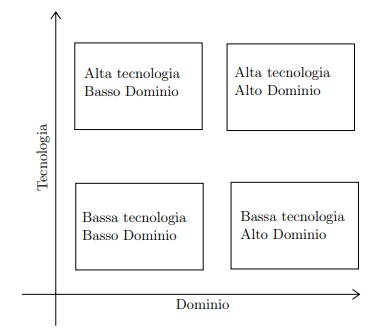
\includegraphics[scale=0.7]{img/varie/valutatori.jpeg}
\end{figure}
Ricordandoci "la regola di \textbf{Nielsen}", abbiamo scelto 5 tester per l'applicaizone. I 5 utenti metteranno in evidenza la maggior parte dei problemi di usabilità (circa il 75\%) più significativi (aggiungerne di più comporterebbe un aumento dei costi inutile). Gli utenti sono i seguenti:
\begin{itemize}
  \item \textbf{Valutatore}: con bassa conoscenza tecnologica, bassa conoscenza del dominio (Fabiana E.).
  \item \textbf{Valutatori} x2: bassa conoscenza tecnologica, alta conoscenza del dominio
        \subitem (Antonio L., Roberto P.).
  \item \textbf{Valutatore}: con alta conoscenza tecnologica, bassa conoscenza del dominio (Corrado R.).
  \item \textbf{Valutatore}: con alta conoscenza tecnologica, alta conoscenza del dominio (Ciro C.).
\end{itemize}
\`{E} importante che gli utenti scelti (al di fuori del gruppo di progetto, in modo da non avere risultati falsati) abbiano caratteristiche diverse, scelti con cura in modo da rappresentare la più ampia fascia d'utenti (per quanto possibile).
\newpage
\subsubsection{Tecnica utilizzata}
Per lo svolgimento dei test è stato utilizzata la tecnica del \textit{Mago di Oz}, che consiste nel realizzare un prototipo interattivo, in cui le risposte, se possibile all'insaputa dell'utente, da parte di un essere umano che operi "dietro le quinte". nella maniera più fedele possibile.
\paragraph{Compiti assegnati} Ai nostri utenti sono stati assegnati i seguenti 4 compiti da svolgere:
\begin{itemize}
  \item \textbf{Compito 1}: Cambio password.
  \item \textbf{Compito 2}: Creazione piatto.
  \item \textbf{Compito 3}: Cancellazione piatto.
  \item \textbf{Compito 4}: Visualizzazione notifica.
\end{itemize}
Nella seguente tabella è possibile visualizzare i risultati dei test:
\begin{table}[H]
  \begin{center}
    \def\arraystretch{1.5}
    \begin{tabular}{|l|c|c|c|c|}
      \hline
      &\textbf{COMPITO 1} & \textbf{COMPITO 2} & \textbf{COMPITO 3} & \textbf{COMPITO 4} \\
      \hline
      \textbf{Fabiana E.} & S                & S              & S                  & P                \\
      \hline
      \textbf{Antonio L.} & S                & F              & S                  & S                \\
      \hline
      \textbf{Roberto P.} & S                & S              & S                  & S                \\
      \hline
      \textbf{Corrado R.} & S                & P              & P                  & S                \\
      \hline
      \textbf{Ciro C.} & S                & P              & S                  & S                \\
      \hline
    \end{tabular}
  \end{center}
  \caption{F = fallimento = 0; P = successo parziale = 0.5; S = successo = 1}
\end{table}
Avendo cosi un totale di $17/20 = (15+(4*0.5))$ compiti eseguiti per una percentuale di $85\%$.
\paragraph{Feedback degli utenti} i nostri tester ci hanno evidenziato come:
\begin{itemize}
  \item L'inserimento del prezzo era lento e incline ad errori, abbiamo sostituito così l'inserimento a mo' di orario con un semplice EditText.
  \item La visualizzazione delle notifiche era controintuitiva a primo impatto, infatti non tutti sono riusciti subito a trovare il tasto "visualizza", adesso con un semplice tocco della notifica appare il tasto "visualizza". 
\end{itemize} 
\paragraph{P.S.} in principio erano stati assegnati dei punteggi anche al tempo impiegato, abbiamo però notato che il nostro gruppo di tester si aggirava più o meno sullo stesso tempo impiegato, abbiamo quindi deciso fosse inutile (nel nostro caso) lasciare quei punteggi.